\documentclass[../../InformazioneQuantistica.tex]{subfiles}
\begin{document}

\section{Phase Estimation Algorithm}
\lesson{16 \greendot}{6/6/2019}

Consideriamo una trasformazione unitaria $U$ che agisce \q{aggiungendo una fase} $\phi$ ad un suo autovettore $\ket{u}$:
\begin{align*}
U\ket{u} = e^{i\phi}\ket{u} \quad 0\leq \phi \leq 2\pi
\end{align*}

Supponiamo di poter preparare lo stato $\ket{u}$ con un registro di $m$ qubit, e di avere a disposizione delle porte logiche \textit{Control}-$U^{2^J}$, con $J\geq 0$, capaci di applicare condizionalmente (ossia a seconda del valore di certi qubit di controllo) la trasformazione $U$ reiterata $2^J$ volte.\\
Come possiamo \textit{stimare} la fase $\phi$?\\

In primo luogo, non possiamo misurare direttamente lo stato trasformato $e^{i\phi}\ket{u}$, dato che differisce da $\ket{u}$ per una sola fase globale - e quindi produce gli stessi valori attesi per ogni osservabile indipendentemente dal valore di $\phi$.\\
Tuttavia, utilizzando i \textit{gate} di controllo a nostra disposizione è possibile \textit{trasformare} la fase globale in una fase relativa, e quindi creare un algoritmo per ottenere una stima arbitrariamente vicina a $\phi$.\\
Nello specifico, possiamo determinare $n$ bit di $\phi$, ossia un numero $a = a_{n-1} a_{n-2} \dots a_1 a_0$ di $n$ bit tale che:
\begin{align}
\phi = 2\pi \left(\frac{a}{2^n} + \delta \right); \qquad 0 \leq |\delta| \leq \frac{1}{2^{n+1}}
\label{eqn:phi}
\end{align}
dove $\delta$ è l'\textit{errore} associato ad $a$, che diminuisce esponenzialmente al crescere del numero $n$ di bit utilizzati. In questa notazione, denotiamo con $\tilde{\phi}$ la miglior stima della fase, e con $\delta \phi$ il relativo errore:
\begin{align*}
    \tilde{\phi} = 2\pi \frac{a}{2^n}; \qquad \delta\phi = 2\pi \delta; \qquad \phi = \tilde{\phi} + \delta\phi
\end{align*}

Per ottener ciò, facciamo uso del seguente circuito quantistico:
\begin{figure}[H]
\centering
\begin{quantikz}[row sep=0.2cm]
\lstick[wires=5]{$\ket{0}^{\otimes n}$} \slice{$\ket{\Psi_0}$} & \gate{H} \slice{$\ket{\Psi_1}$} & \qw & \qw & \qw & \qw & \qw & \ctrl{5} \slice{$\ket{\Psi_2}$}& \gate[5, nwires={3}]{\op{QFT}^{-1}} \slice{$\ket{\Psi_3}$}& \meter{} \qw\\
 & \gate{H} & \qw & \qw & \qw & \qw & \ctrl{4} & \qw & \qw & \meter{} \qw\\
 & \ \vdots \  & & & & & & & &  \meter{} \qwbundle[alternate]{}\\
& \gate{H} & \qw & \qw & \ctrl{2} & \qw & \qw & \qw & \qw & \meter{} \qw \\
 & \gate{H} & \qw & \ctrl{1} & \qw & \qw & \qw & \qw & \qw & \meter{} \qw \\
\lstick{$\ket{u}$} & \qwbundle[alternate]{} & \qwbundle[alternate]{} & \gate{U^{2^0}} \qwbundle[alternate]{} & \gate{U^{2^1}}\qwbundle[alternate]{} & \ \push{\ldots}\  \qwbundle[alternate]{} & \gate{U^{2^{n-2}}} \qwbundle[alternate]{} & \gate{U^{2^{n-1}}} \qwbundle[alternate]{} & \qwbundle[alternate]{} & \qwbundle[alternate]{}
\end{quantikz}
\caption{Schema a porte logiche quantistiche dell'algoritmo di Phase Estimation\label{fig:phase-estimation-gate}}
\end{figure}

Impieghiamo due registri: uno da $n$ qubit, inizializzato a $\ket{0}$, che conterrà la stima $a$ della fase, e uno da $m$ qubit, inizializzato a $\ket{u}$, su cui agiscono le $C-U^{2^J}$. Lo stato iniziale è perciò:
\begin{align*}
\ket{\Psi_0} = (\underbrace{\ket{0}\ket{0}\cdots \ket{0}}_{n})_1 \otimes \underbrace{\ket{u}_2}_m
\end{align*}

Tramite $n$ Hadamard realizziamo una sovrapposizione di tutti gli stati nel primo registro:
\begin{align*}
    \ket{\Psi_1} = (H^{\otimes n} \otimes \bb{I}^m ) \ket{\Psi_0} = \left( \frac{1}{\sqrt{2}} \otimes_{i=1}^n (\ket{0} + \ket{1})_1 \right)  \otimes \ket{u}_2
\end{align*}

A questo punto, applichiamo in sequenza $n$ C-$U^{2^J}$ sul secondo registro, ciascuna condizionata da uno degli $n$ qubit del primo, giungendo allo stato $\ket{\Psi_2}$. Partiamo calcolando l'azione di C-$U^{2^J}$ sullo stato $(\ket{0}+\ket{1})/\sqrt{2}\otimes\ket{u}$:
\begin{align} \nonumber
\underbrace{\op{C-U}^{2^J}}_{W} \left[\frac{1}{\sqrt{2}}(\ket{0}+\ket{1})\otimes \ket{u}\right] &= \frac{1}{\sqrt{2}} \left[W\ket{0}\ket{u} + W\ket{1}\ket{u}\right] = \\ \nonumber
&= \frac{1}{\sqrt{2}}\left[\ket{0}\ket{u} + \exp\left(i2^J \phi\right) \ket{1}\ket{u}\right] =\\
&=\frac{1}{\sqrt{2}}\left[ \ket{0} + \exp\left( i 2^J \phi \right) \ket{1} \right] \otimes \ket{u}
\label{eqn:C-U}
\end{align}
Notiamo che, poiché $\ket{u}$ è autovalore di $U$, $U^2$, $U^4$..., la C-$U^{2^J}$ non modifica lo stato del secondo registro, mentre propaga una fase relativa (misurabile) nello stato del primo registro. Poiché allora l'input di ciascuna C-$U^{2^J}$ non cambia, basta reiterare la (\ref{eqn:C-U}) per ottenere $\ket{\Psi_2}$:
\begin{align} \nonumber
\ket{\Psi_2} &= \frac{1}{\sqrt{2^n}} \left( \ket{0} + \exp\left(i \phi 2^{n-1}\right) \ket{1}\right) \left(\ket{0} + \exp\left( i \phi 2^{n-2}\right) \ket{1}\right) \otimes \cdots\\ \nonumber
&\qquad \cdots \otimes \left( \ket{0} + e^{i2\phi} \ket{1}\right)\left( \ket{0} + e^{i\phi}\ket{1}\right) \otimes \ket{u} =\\ \nonumber 
&= \frac{1}{\sqrt{2^n}}\left( \ket{0}\ket{0}\cdots \ket{0} + e^{i\phi}\ket{0}\cdots \ket{0}\ket{1} + \cdots 
\exp({i(2^n-1)\phi})\ket{1}\ket{1}\cdots \ket{1} \right)_1 \otimes \ket{u}_2 = \\
&= \frac{1}{\sqrt{2^n}} \sum_{y=0}^{2^n-1} e^{i\phi y} \ket{y}_1\ket{u}_2 \label{eqn:qftpsi}
\end{align}
Concentriamoci sullo stato del solo primo registro. La (\ref{eqn:qftpsi}) ha la forma della trasformata di Fourier dello stato $\ket{\phi}$ che codifica la fase. Per determinarlo, perciò, applichiamo l'inversa della \textit{Quantum Fourier Transform}, che è definita da:
\begin{align*}
\op{QFT}^{-1}\{\ket{y}\} = \frac{1}{\sqrt{2^n}} \sum_{x=0}^{2^{n}-1} \exp\left(-\frac{2\pi i xy}{2^n}\right) \ket{x}
\end{align*}

Otteniamo allora (per il primo registro):
\begin{align*}
    \ket{\Psi_3} &= \op{QFT}^{-1}\{\ket{\Psi_2}\} = \frac{1}{2^n} \sum_{x=0}^{2^n-1} \sum_{y=0}^{2^n-1} \exp\left(-\frac{2\pi i xy}{2^n}\right) \hlc{Yellow}{e^{i\phi y}} \ket{x} = \\
    & \underset{(\ref{eqn:phi})}{=} \frac{1}{2^n} \sum_{x=0}^{2^n-1} \sum_{y=0}^{2^n-1} \exp\left(-\frac{2\pi i xy}{2^n}\right) \hlc{Yellow}{\exp\left( \frac{2\pi i ay}{2^n}\right) \exp(2\pi i \delta y)} \ket{x} =\\
    &= \frac{1}{2^n} \sum_{x=0}^{2^n-1} \sum_{y=0}^{2^n-1} \exp\left( -\frac{2\pi i y}{2^n}(x-a) \right) \exp(2\pi i \delta y ) \ket{x}
\end{align*}

Una misura proiettiva risulta in un certo valore $b$ con probabilità:
\begin{align*}
   P(b) = |\braket{b|\Psi_3}|^2 = \left| \frac{1}{2^n} \sum_{y=0}^{2^n-1} \exp\left(-\frac{2\pi i xy}{2^n} (b-a) \right) \exp(2\pi i \delta y ) \right|^2
\end{align*}
dato che $\braket{b|x} = \delta_{xb}$.\\
Distinguiamo ora tra due casi:
\begin{enumerate}
    \item Se $\delta = 0$, ossia se $\ket{\phi}$ può essere \textit{codificata} da $n$ bit (o meno), allora vi è un solo valore di $b$ con probabilità non nulla, ed è quello che corrisponde alla miglior stima $a$. Infatti:
    \begin{align*}
        P(b=a) = \left| \frac{1}{2^n} 2^n \right| = 1
    \end{align*}
    \item Se $\delta \neq 0$, sono in generale possibili più risultati. Quello che offre la stima corretta di $\phi$, ossia $b=a$, ha probabilità data da:
    \begin{align} \nonumber
        P(b=a) &= \left|\frac{1}{2^n} \sum_{y=0}^{2^n-1} \exp(2\pi i \delta y ) \right|^2 = \frac{1}{2^{2^n}} \left| \sum_{y=0}^{2^n-1} \big[\underbrace{\exp(2\pi i \delta)}_\alpha\big]^y \right |^2 =\\ \nonumber
        &\underset{(a)}{=} \frac{1}{2^{2^n}} \left| \frac{1-\alpha^{2^n}}{1-\alpha} \right|^2 = \frac{1}{2^{2n}} \left| \frac{1-\exp(2\pi i \delta 2^n)}{1-\exp(2\pi i \delta )}\right|^2 = \\
        &\underset{(b)}{=} \frac{1}{2^{2n}} \left| \frac{\sin(\pi \delta 2^n)}{\sin(\pi\delta)} \right|^2
        \label{eqn:Pba-deltaneq0}
    \end{align}
    dove in (a) si è usata la formula per le somme parziali di una serie geometrica:
    \begin{align*}
        \sum_{k=0}^n x^k = \frac{1-x^{n+1}}{1-x}
    \end{align*}
    e in (b) un'identità dell'esponenziale complesso:
    \begin{align*}
        |1-\exp A | &= |1-\cos A -i \sin A| = \sqrt{(1-\cos A)^2 + \sin^2 A} =\\
        &=\sqrt{2} \frac{\sqrt{1-\cos A}}{\textcolor{Red}{\sqrt{2}}}\textcolor{Red}{\sqrt{2}} = 2\sin \frac{A}{2}
    \end{align*}
    
    Diamo una stima di $P(b=a)$. Poiché $2z \leq \sin(\pi z) \leq \pi z$ $\forall z \in [0,1/2]$, si ha:
    \begin{align*}
        |\sin(\pi \delta 2^n)| \geq 2 |\delta| 2^n; \qquad |\sin(\pi \delta)| \leq \pi |\delta|
    \end{align*}
    Sostituendo in (\ref{eqn:Pba-deltaneq0}) otteniamo:
    \begin{align*}
        P(b=a) \geq \frac{1}{2^{2n}} \frac{4|\delta|^2 2^{2n}}{ \pi^2 |\delta|^2} = \frac{4}{\pi^2} \approx 0.405
    \end{align*}
    Perciò la miglior stima $a$ di $n$ bit di $\phi$ si ottiene con una buona probabilità.\\
    Si può dimostrare che gli altri esiti probabili differiscono da $a$ per i bit meno significativi. Nello specifico, si possono ottenere $l$ bit della fase $\phi$ con una probabilità $p>1-\epsilon$ usando $n=l+O(\log(1/\epsilon))$ qubit.\\
    Numericamente, con \textit{soli} $60$ qubit si raggiungono stime con $18$ cifre significative - comparabili con le migliori misure tecnologicamente possibili nella fisica sperimentale.
\end{enumerate}

\section{Eigensolver}
Un'applicazione importante dell'algoritmo di Phase Estimation è legata al calcolo di autovalori e autofunzioni di una certa Hamiltoniana $H$ \textit{indipendente dal tempo}.\\
Lavorando in rappresentazione $\{x\}$ (con $d=1$ per semplicità), denotiamo con $\phi_\alpha(x)$ le autofunzioni di $H$ di autovalore $\mathcal{E}_\alpha$, tali che:
\begin{align*}
    H\phi_\alpha(x) = \mathcal{E}_\alpha \phi_\alpha(x) \quad \alpha \in \bb{N}
\end{align*}
L'evoluzione temporale di tali autostati avviene per l'aggiunta di una fase:
\begin{align*}
    \phi_\alpha(x,t=0) \underset{U(t)}{\mapsto} \phi_\alpha(x,t) = \exp\left(-\frac{i}{\hbar} t \mathcal{E}_\alpha\right) \phi_\alpha(x,0)
\end{align*}
Ciò deriva direttamente dall'equazione di Schr\"odinger dipendente dal tempo, che per una generica funzione d'onda $\psi(x,t)$ è data da:
\begin{align*}
    i\hbar \frac{\partial}{\partial t} \psi(x,t) = H(x) \psi(x,t)
\end{align*}
Perciò gli autovettori $\phi_\alpha(x)$ sono anche autovettori dell'operatore $U(t)$ di evoluzione temporale, che ha le stesse caratteristiche dell'operatore $U$ visto nella sezione precedente:
\begin{align*}
    U(t) = \exp\left(-\frac{i}{\hbar} H t\right); \qquad U(t)\ket{\phi_\alpha} = \exp\left(-\frac{i}{\hbar}t \mathcal{E}_\alpha\right) \ket{\phi_\alpha}
\end{align*}

\subsection{Algoritmo classico}
Classicamente, un algoritmo che permette di trovare autovalori e autovettori (e che, come vedremo, può essere adattato al caso quantistico con un certo guadagno computazionale) si basa sul calcolo di trasformate di Fourier.\\
Consideriamo una finestra temporale finita $0\leq t \leq \bar{t}$, e una funzione d'onda iniziale arbitraria $\psi_0(x)$, che scriviamo nella base degli autostati di $H$:
\begin{align*}
    \psi_0(x) \equiv \psi(x,t=0) = \sum_{\alpha=0}^{+\infty} a_\alpha \phi_\alpha(x)
\end{align*}
La sua evoluzione temporale ad un certo istante $t$ è quindi data da:
\begin{align*}
    \psi_0(x,t) = \sum_{\alpha=0}^{+\infty} a_\alpha \exp\left( - \frac{i}{\hbar} \mathcal{E}_\alpha t \right) \phi_\alpha(x) = \sum_{\alpha=0}^{+\infty} a_\alpha e^{-i\omega_\alpha t} \phi_\alpha(x); \qquad \omega_\alpha = \frac{\mathcal{E}_\alpha}{\hbar}
\end{align*}
Fissiamo un punto $x=x_0$. La funzione $\psi(x_0,t)$ è la sovrapposizione di funzioni periodiche con pulsazioni $\omega_\alpha$, che possono essere evidenziate svolgendo una trasformata di Fourier\footnote{Gli integrali possono essere calcolati numericamente \textit{discretizzando} il dominio}:
\begin{align*}
    \tilde{\psi}(x_0, \omega) &= \mathcal{F}[\psi(x_0,t)](x_0, \omega) =\\
    &= \int_0^{\bar{t}} dt\, e^{i\omega t} \sum_{\alpha=0}^{+\infty} a_\alpha e^{-i\omega_\alpha t}\phi_\alpha(x_0) = 
    \sum_{\alpha=0}^{+\infty} a_\alpha \int_0^{\bar{t}} dt\, \exp(i(\omega-\omega_\alpha)t) \phi_\alpha(x)
\end{align*}
Quando $\omega = \omega_{\bar{\alpha}}$ otteniamo:
\begin{align*}
    \tilde{\psi}(x_0, \omega_{\bar{\alpha}}) = a_{\bar{\alpha}} \phi_{\bar{\alpha}}(x_0) \bar{t} + \sum_{\alpha \neq \bar{\alpha}} a_\alpha \int_0^{\bar{t}} dt\, \exp(i(\omega-\omega_\alpha)t)\phi_\alpha(x)
\end{align*}
Per $\bar{t}$ sufficientemente grande ($\bar{t} \gg \omega_{\bar{\alpha}}/(2\pi)$) il secondo termine è la somma di integrali di funzioni oscillanti su un numero grande di oscillazioni, ed è perciò limitato (è $\to 0$), mentre il primo termine scala linearmente con $\bar{t}$. Del resto, per i \textit{punti intermedi} (in cui $\omega \neq \omega_\alpha \forall \alpha$), la funzione è solamente limitata. Deduciamo perciò che $\tilde{\psi}(x_0, \omega)$ è piccata sulle $\omega_\alpha$ (figura \ref{fig:Fourier-transform-ex}).\\
Dai massimi di $\tilde\psi(x_0, \omega)$ è perciò possibile stimare le $\omega_\alpha$ e quindi gli autovalori\footnote{Più precisamente, tale metodo consente di determinare solo gli autovalori per cui $a_\alpha \neq 0$, ossia $\braket{\psi_0|\phi_\alpha} \neq 0$. Per una funzione d'onda iniziale generica, senza particolari simmetrie, in genere $a_\alpha \neq 0$ è verificata.} $\mathcal{E}_\alpha$ di $H$. Per le autofunzioni, notiamo che per $\bar{t}$ sufficientemente grande:
\begin{align*}
    \frac{1}{\bar{t}} \tilde{\psi}(x_0, \omega_{\bar{\alpha}}) \approx a_{\bar{\alpha}} \phi_{\bar{\alpha}}(x_0)
\end{align*}
Perciò:
\begin{align*}
    \frac{\tilde{\psi}(x_1, \omega_{\bar{\alpha}})}
    {\tilde{\psi}(x_2, \omega_{\bar{\alpha}})} = 
    \frac{\phi_{\bar{\alpha}}(x_1)}{\phi_{\bar{\alpha}}(x_2)}
\end{align*}
Fissando arbitrariamente $\phi_{\bar{\alpha}}(x_1) \overset{!}{=} 1$ si può valutare l'autofunzione $\bar{\alpha}$-esima in qualsiasi altro punto - a meno della normalizzazione (che può essere imposta successivamente).\\ \marginpar{Discretizzazione del problema}
Poiché le risorse computazionali sono finite, nella pratica ci si limita ad una certa regione, per esempio $x\in [-L,L]$ per un certo $L$ fissato, che viene \textit{discretizzato}, ossia suddiviso in $2^n$ parti, ciascuna \textit{lunga} $\Delta x = 2L/(2^n-1)$, dove $n$ è il numero di bit a disposizione. Le autofunzioni (così come la funzione d'onda $\psi_0(x)$ iniziale) sono valutate solo nei punti $x_i$ tali che:
\begin{align*}
    x_i = -L + i\Delta x \qquad i\in \{0, \dots, 2^{n}-1\}
\end{align*}

\begin{figure}[H]
\centering
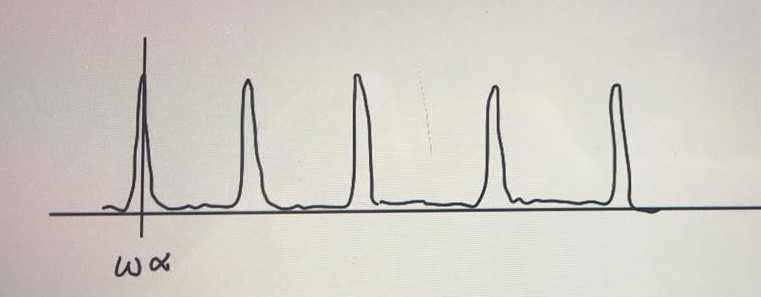
\includegraphics[width=0.7\textwidth]{Immagini/6_6/Fourier.jpg}
\caption{Plot di esempio della trasformata di Fourier\label{fig:Fourier-transform-ex}}
\end{figure}

\subsection{Algoritmo quantistico}
L'algoritmo appena visto si traduce in modo naturale al caso quantistico. Partiamo da uno stato $\ket{\Psi_0}$ arbitrario, che codifica una funzione d'onda $\psi_0(x)$ \textit{valutata} in $2^n$ punti:
\begin{align*}
\ket{\Psi_0} = \sum_{i=0}^{2^n-1} \psi_0(x_i)\ket{i}
\end{align*}
Notiamo che bastano $n$ qubit per codificare $2^n$ punti della funzione d'onda, con un guadagno esponenziale di memoria (ammesso che sia possibile preparare un tale stato).\\
Per semplicità (di calcolo e di implementazione), scegliamo $\ket{\psi_0}$ come un vettore casuale della base computazionale:
\begin{align*}
    \ket{\psi_0} \overset{!}{=} \ket{\bar{j}}
\end{align*}
che corrisponde ad una funzione d'onda $\psi_0(x) = \delta_{x x_{\bar{j}}}$ \q{localizzata in un punto}.\\

L'algoritmo è lo stesso usato per la Phase-Estimation, dove ora $\ket{\psi_0}$ gioca il ruolo di $\ket{u}$. Supponiamo di avere a disposizione delle gate C-$U^{2^J}$, dove $U$ è l'operatore di evoluzione temporale per un tempo $\Delta t = \bar{t}/(2^{n}-1)$:
\begin{align*}
U = \exp\left(-i H \frac{\Delta t}{\hbar}\right)
\end{align*}
Fortunatamente tali $U$ ammettono un'implementazione efficiente per una larga classe di Hamiltoniane.\\

Prepariamo allora lo stato iniziale:
\begin{align*}
    \ket{\Psi_0} = \ket{0}^{\otimes n}_1 \otimes \ket{\psi_0}_2
\end{align*}
Realizziamo la sovrapposizione massima degli stati dei qubit di controllo (primo registro):
\begin{align*}
    \ket{\Psi_1} = \left(\frac{1}{\sqrt{2^n}} \sum_{j=1}^{2^n-1} \ket{j}_1 \right) \otimes \ket{\psi_0}_2
\end{align*}
E applichiamo la successione delle $n$ C-$U^{2^J}$, giungendo allo stato entangled analogo al (\ref{eqn:qftpsi}):
\begin{align*}
    \ket{\Psi_2} &= \frac{1}{\sqrt{2^n}} \sum_{j=0}^{2^n-1} \ket{j}_1 U^j \ket{\psi_0}_2 \underset{(a)}{=} \frac{1}{\sqrt{2^n}} \sum_{j=0}^{2^n-1} \ket{j}_1 \ket{\psi(j\Delta t)} =\\
    &\underset{(b)}{=} \frac{1}{\sqrt{2^n}}\sum_{j=0}^{2^n-1} \ket{j}_1 \left( \sum_{\alpha=0}^{+\infty} a_\alpha \exp(-i\omega_\alpha j \Delta t) \ket{\phi_\alpha} \right)_2
\end{align*}
dove in (a) abbiamo applicato la definizione dell'operatore di evoluzione temporale, e in (b) siamo passati nella base degli autoket $\ket{\phi_a}$ di $H$.\\
Non resta allora che eseguire una QFT$^{-1}$ sul primo registro. Misurando i primi $n$ qubit si ottiene una stima di una $\omega_{\bar{\alpha}}$ (con probabilità $|a_\alpha|^2$), e immediatamente si fa collassare il secondo registro nel relativo autostato $\ket{\phi_{\bar{\alpha}}}$ (che può essere ricostruito da ulteriori misurazioni).\\
Semplicemente ripetendo l'esecuzione si possono ottenere altri valori di $\omega_\alpha$.\\
Il vantaggio di tutto ciò è che la QFT è molto più efficiente dell'analogo classico. Perciò, a meno di aver scelto una $\ket{\psi_0}$ con proiezione troppo piccola lungo un $\ket{\phi_\alpha}$ desiderato, si possono calcolare tutti gli autovalori nella regione di interesse (per esempio alle energie prossime allo stato fondamentale) in tempo polinomiale.
%https://quantumalgorithmzoo.org/

\section{Error correction}
Ogni sistema è soggetto a \textit{malfunzionamenti}, e ogni implementazione può - a seguito di determinati eventi più o meno rari - produrre \textit{errori}. Risulta quindi importante studiare il modo di \textit{ridurre quanto più possibile} tali evenienze, ed eventualmente \textit{correggere comportamenti anomali}. Analizziamo ora alcuni metodi che permettono di raggiungere questi obiettivi.

\subsection{Classical error correction}
Sia $\epsilon$ la probabilità che un qualsiasi generico protocollo generi un \textit{errore}. Per una buona implementazione $\epsilon \ll 1$, ma comunque $\neq 0$. Ridurre ulteriormente $\epsilon$ può però risultare molto costoso o difficile. Una strategia migliore è allora quella di inserire \textbf{ridondanza} nella comunicazione, dando così la possibilità al destinatario di rilevare e correggere alcuni tipi di errori.\\

Consideriamo, per esempio, una situazione in cui Alice vuole mandare un bit $a \in \{0,1\}$ a Bob. Avremo allora una probabilità $\epsilon$ che Bob riceva un bit diverso da quello spedito da Alice, a seguito di un qualche fallimento del canale di trasmissione.\\
Se però Alice invia $3$ copie del bit a Bob, per esempio $000$, un singolo errore con $p=\epsilon$ produce un messaggio tra $001$, $010$ e $100$. In tutti e tre i casi Bob può \textit{ricostruire} il messaggio originale applicando il principio del \textbf{voto di maggioranza}: poiché la probabilità $\epsilon$ che un bit sia corrotto è bassa, ci aspettiamo che la maggior parte dei bit siano corretti, e perciò che il messaggio originale sia quello compatibile con la maggior parte dei bit ricevuti - ossia $0$.\\
Tale schema non funziona in ogni caso. Per esempio, se il messaggio originale è $000$ e si verificano $2$ errori, Bob riceve $011$, $101$ o $110$. Applicando il \textit{voto di maggioranza} si ricostruire un messaggio ($1$) diverso da quello originale ($0$). Tuttavia, poiché tale situazione si verifica con probabilità decisamente inferiore, la strategia rimane valida per garantire una maggiore \textit{stabilità} del canale di comunicazione. Lo si può vedere esaminando tutti i casi possibili:
\begin{table}[H]
\centering
\begin{tabular}{lrrr} \toprule
\# Errori & Messaggio ricevuto & Prob. & Fallimento? \\ \midrule
0 & 000 & $(1-\epsilon)^3$ & N\\
1 & 100, 010, 001 & $\epsilon(1-\epsilon)^2$ & N\\
2 & 110, 011, 101 & $\epsilon^2 (1-\epsilon)$ & S\\
3 & 111 & $\epsilon^3$ & S \\ \bottomrule
\end{tabular}
\caption{Esiti possibili per il trasferimento di un bit con un fattore $3$ di ridondanza}
\end{table}
Mettendo tutto insieme, la probabilità di fallimento $P_F^3$ con $3$ bit di ridondanza è data da:
\begin{align*}
P_F^3 = 3[\epsilon^2 (1-\epsilon)]+\epsilon^3 = O(\epsilon^2)
\end{align*}
che è decisamente inferiore rispetto alla probabilità di fallimento per il protocollo a un \textit{solo bit}: $P_F^1 = \epsilon$.

\subsection{Quantum error correction}
Proviamo ad applicare il protocollo di \q{ridondanza + voto} nel caso quantistico. Si rivelano subito alcuni problemi:
\begin{enumerate}
\item Innanzitutto non possiamo \textbf{copiare} $n$ volte uno stato generico $\ket{\psi}$ sconosciuto (no cloning theorem) per generare ridondanza
\item Non è possibile \textbf{misurare} direttamente i qubit ricevuti per confrontarli tra loro, dato che una misura proiettiva modifica irrimediabilmente lo stato a cui si applica
\item Non è detto che gli errori consistano solamente nel \textit{bit-flip}, ossia nella trasformazione di $\ket{0}\leftrightarrow \ket{1}$. Potrebbero esserci effetti, per esempio, che \textit{modificano} la fase relativa tra le due componenti del qubit inviato.
\end{enumerate}

\subsubsection{Quantum bit-flip code}
Supponiamo che Alice voglia inviare un qubit nello stato $\ket{\psi} = \alpha \ket{0} + \beta\ket{1}$ a Bob tramite un canale quantistico affetto da \textbf{rumore}. Supponiamo inoltre che il rumore agisca \textbf{indipendentemente} su ciascun qubit, lasciando un qubit invariato con probabilità $1-\epsilon$, o invertendolo (come un gate NOT, $\sigma_x$) con probabilità $\epsilon$.\\
In tale situazione, introduciamo un protocollo di correzione detto \textbf{3-qubit bit-flip code}, che si basa sul codificare gli stati della base computazionale inserendo \textit{ridondanza}:
\begin{align*}
    \ket{0}\mapsto \ket{\tilde{0}} = \ket{000}; \qquad \ket{1}\mapsto \ket{\tilde{1}} = \ket{111}
\end{align*}
Alice, perciò, applica tale codifica al proprio qubit $\ket{\psi}$:
\begin{align*}
    \ket{\psi} = \alpha\ket{0} + \beta \ket{1} \mapsto \ket{\tilde{\psi}} = \alpha \ket{\tilde{0}} + \beta \ket{\tilde{1}}
\end{align*}
Notiamo che:
\begin{align*}
    \ket{\tilde{\psi}} = \alpha\ket{000} + \beta\ket{111} \neq \ket{\psi}\ket{\psi}\ket{\psi} = (\alpha\ket{0} + \beta\ket{1})\otimes (\alpha\ket{0} + \beta\ket{1})\otimes (\alpha \ket{0} + \beta\ket{1})
\end{align*}
e perciò la codifica \textbf{non viola} il teorema del no-cloning, e infatti può essere implementata utilizzando due CNOT (figura \ref{fig:ridondanza-gate}).


\begin{comment}
Partiamo dagli stati iniziali. Risulta semplice convertire gli stati di base:
\begin{align*}
\ket{0} &\to \ket{\tilde{0}} = \ket{0}\ket{0}\ket{0}\\
\ket{1} &\to \ket{\tilde{1}} = \ket{1}\ket{1}\ket{1}
\end{align*}
In generale, però, convertire una funzione d'onda generica non è altrettanto semplice:
\begin{align*}
\ket{\psi} = \alpha \ket{0} + \beta\ket{1} \to \alpha \ket{\tilde{0}} + \beta \ket{\tilde{1}} = \alpha \ket{0}\ket{0}\ket{0} + \beta \ket{1}\ket{1}\ket{1}
\end{align*}
e quindi non è immediato generalizzare a $n$ qubit tale protocollo (come invece si può fare nel caso classico).\\
\textbf{Nota}: lo stato \q{ridondante} è decisamente diverso dal \textit{clonare} lo stato iniziale:
\begin{align*}
(\alpha \ket{0} + \beta \ket{1})(\alpha \ket{0} + \beta \ket{1})(\alpha \ket{0} + \beta \ket{1}) \neq \alpha \ket{000}+\beta \ket{111}
\end{align*}
\end{comment}

\begin{figure}[H]
\centering
\begin{quantikz}
\lstick{$\ket{\psi}$} & \ctrl{1} & \ctrl{2} & \qw \rstick[wires=3]{$\ket{\tilde{\psi}}$}\\
\lstick{$\ket{0}$} & \targ{} & \qw & \qw\\
\lstick{$\ket{0}$} & \qw & \targ{} & \qw 
\end{quantikz}
\caption{Schema a porte logiche quantistiche per la generazione di ridondanza\label{fig:ridondanza-gate}}
\end{figure}

Consideriamo tutte le possibili combinazioni di errore (date le ipotesi):
\begin{table}[H]
\centering
\begin{tabular}{llll}\toprule
\textbf{Messaggio Ricevuto} & \textbf{Prob.} & \textbf{Stato finale} & $\ket{x_0}\ket{x_1}$ \\ \midrule $\alpha \ket{000}+\beta\ket{111}$ & $(1-\epsilon)^3$ & $\textcolor{ForestGreen}{\alpha \ket{000} + \beta\ket{111}}$ & $\ket{00}$\\
$\alpha \ket{100}+ \beta\ket{011}$ & $\epsilon(1-\epsilon)^2$  & $\textcolor{ForestGreen}{\alpha \ket{000} + \beta\ket{111}}$ & $\ket{11}$\\
$\alpha \ket{010} + \beta\ket{101}$ & $\epsilon(1-\epsilon)^2$ & $\textcolor{ForestGreen}{\alpha \ket{000} + \beta\ket{111}}$ & $\ket{10}$ \\
$\alpha \ket{001} + \beta \ket{110}$ & $\epsilon(1-\epsilon)^2$ & $\textcolor{ForestGreen}{\alpha \ket{000} + \beta\ket{111}}$ & $\ket{01}$\\
$\alpha \ket{110} + \beta\ket{001}$ & $\epsilon^2 (1-\epsilon)$ &$\textcolor{Red}{\alpha \ket{111}+\beta\ket{000}}$ & $\ket{01}$ \\
$\alpha\ket{101} + \beta\ket{100}$ & $\epsilon^2 (1-\epsilon)$ & $\textcolor{Red}{\alpha \ket{111}+\beta\ket{000}}$ & $\ket{10}$\\
$\alpha\ket{011} + \beta\ket{100}$ & $\epsilon^2 (1-\epsilon)$ & $\textcolor{Red}{\alpha \ket{111}+\beta\ket{000}}$ & $\ket{11}$\\
$\alpha \ket{111} + \beta\ket{000}$ & $\epsilon^3$ & $\textcolor{Red}{\alpha \ket{111}+\beta\ket{000}}$ & $\ket{00}$ \\ \bottomrule
\end{tabular}
\caption{Possibili messaggi ricevuti a seguito di errori\label{tab:quantum-3bit}}
\end{table}

Per capire in quale caso ci si trovi non è possibile misurare direttamente i $3$ qubit - ciò distruggerebbe la sovrapposizione coerente dello stato $\ket{\psi}$ che si vuole ricevere.\\
Piuttosto, è possibile \textit{correlare} $2$ qubit ausiliari e misurarli lasciando invariati gli altri $3$, che possono poi essere corretti applicando una certa operazione $U$ determinata dall'informazione ricavata dalle misure.\\
L'idea è la seguente. Ipotizziamo, per esempio, che Bob abbia ricevuto lo stato:
\begin{align*}
    \ket{\Psi_1} = \alpha \ket{100} + \beta\ket{011}
\end{align*}
Bob può usare due qubit ausiliari per misurare la \textit{correlazione} tra $2$ coppie dei $3$ qubit. Nel dettaglio, trova che nello stato ricevuto, primo e secondo qubit differiscono, così come il primo e il terzo. Nell'ipotesi (probabile) che vi sia stato un solo errore, una coppia di qubit differenti indica che uno dei due è quello errato. In questo caso, perciò, le informazioni ricavate puntano sul primo qubit - che può quindi essere corretto mediante un NOT ($\sigma_x$).\\

L'operazione appena discussa è realizzata dal circuito di figura \ref{fig:bit-ausiliari}. L'idea di base è che una sequenza di due CNOT che usano come controllo qubit nello \textbf{stesso} stato equivale ad un'identità, dato che non è altro che l'applicazione di una stessa \textit{trasformazione unitaria} ripetuta due volte.\\
D'altro canto, due CNOT che partono da stati $\ket{\psi}$ e $\sigma_x \ket{\psi}$ equivalgono a un'unica NOT.


\begin{figure}[H]
\centering
\begin{quantikz}
\lstick[wires=3]{$\ket{\Psi_1}$} & \ctrl{3} & \qw & \ctrl{4} & \qw  \rstick[wires=3]{$\ket{\Psi_1}$}\\
& \qw & \ctrl{2} & \qw & \qw\\
& \qw & \qw & \qw & \ctrl{2} \\
\lstick{$\ket{0}$} & \targ{} & \targ{} & \qw & \qw & \meter{} \qw & \rstick{$\ket{x_0}$}\\
\lstick{$\ket{0}$} & \qw & \qw & \targ{} & \targ{} & \meter{} \qw & \rstick{$\ket{x_1}$}
\end{quantikz}
\caption{Schema a porte logiche quantistiche per la misura di correlazioni tra i qubit ridondanti\label{fig:bit-ausiliari}}
\end{figure}

A seconda degli stati $\ket{x_0}\ket{x_1}$ misurati possiamo correggere opportunamente l'errore rilevato, come mostrato in tabella \ref{tab:quantum-3bit}. Notiamo che a volte la correzione non consente di ricavare lo stato originale (esattamente come nel caso classico). Ciò è dovuto al fatto che, potendo misurare solo $2$ correlazioni, possiamo distinguere solo $4$ degli $8$ casi possibili.\\


Uno schema molto simile può essere adottato per correggere errori che consistono in un'\textit{inversione di fase}, ossia tali da mappare:
\begin{align*}
    \ket{+} \mapsto \ket{-}; \qquad \ket{-} \mapsto \ket{+}
\end{align*}
dove:
\begin{align*}
    \ket{+} \equiv \frac{1}{\sqrt{2}}(\ket{0} + \ket{1}); \qquad \ket{-} \equiv \frac{1}{\sqrt{2}}(\ket{0}-\ket{1})
\end{align*}

L'idea è di usare lo stesso circuito, ma partendo da una codifica in una differente base:
\begin{align*}
\ket{0} &\mapsto \ket{+++}\\
\ket{1} &\mapsto \ket{---}
\end{align*}

Un'implementazione per tale codifica è mostrata nella figura \ref{fig:phase-correction}
\begin{figure}
    \centering
    \begin{quantikz}
        \lstick{$\ket{\psi}$} & \ctrl{1} & \ctrl{2} & \gate{H} & \qw \rstick[wires=3]{$\ket{\tilde{\psi}}$}\\
        \lstick{$\ket{0}$} & \targ{} & \qw & \gate{H} & \qw \\
        \lstick{$\ket{0}$} & \qw & \targ{} & \gate{H} & \qw
    \end{quantikz}
    \caption{Circuito a gate quantistici per realizzare la codifica del \textit{3-qubit phase-flip code}}
    \label{fig:phase-correction}
\end{figure}

\subsubsection{Correzioni avanzate}
Generalizzando, possiamo correggere entrambe le tipologie di errori con uno stesso circuito, codificando la ridondanza in $9$ qubit (\textbf{9-qubit Shor code}):
\begin{align*}
\ket{0} &\mapsto \ket{\tilde{0}} = \frac{1}{\sqrt{8}} (\ket{000}+\ket{111})(\ket{000}+\ket{111})(\ket{000}+\ket{111})\\
\ket{1} &\mapsto \ket{\tilde{1}} = \frac{1}{\sqrt{8}} (\ket{000}-\ket{111}) (\ket{000}-\ket{111}) (\ket{000}-\ket{111})
\end{align*}
Le idee sono le stesse di prima, ma la scala del circuito rende il tutto estremamente più complicato.\\

Allo stato attuale si reputa che raggiungendo $\epsilon \approx 10^{-3}\div 10^{-4}$, mediante algoritmi di questo tipo si possa realizzare il \textit{Fault tolerant quantum computing}, ossia un'architettura di computazione quantistica \textit{resistente} a tipologie generali di errore.\\

Un'altra strada per la correzione degli errori è data dal codificare qubit nei sottospazi \textit{invarianti} per le \textit{simmetrie} degli errori possibili.\\
Per esempio, consideriamo un errore che aggiunga una fase:
\begin{align*}
\begin{cases}
\ket{0} \mapsto \ket{0}\\
\ket{1} \mapsto e^{i\phi}\ket{1}
\end{cases}
\end{align*}
L'idea è di codificare $\ket{0}$ e $\ket{1}$ nella sovrapposizione di stati a più qubit che si trovano nello stesso autospazio dell'\textit{operatore errore}. Nel nostro caso, se esaminiamo l'azione dell'errore sui vettori della base computazionale per $2$ qubit, notiamo due stati su cui l'errore agisce \q{nello stesso modo}:
\begin{align*}
\begin{cases}
\ket{00} \mapsto \ket{00}\\
\ket{01} \mapsto e^{i\phi}\ket{01} \equiv \ket{0}\\
\ket{10} \mapsto e^{i\phi}\ket{10} \equiv \ket{1}\\
\ket{11} \mapsto e^{2i\phi} \ket{11}
\end{cases}
\end{align*}
Scegliendo allora $\ket{0} \mapsto \ket{01}$ e $\ket{1} \mapsto \ket{10}$ come codifica, l'azione dell'errore aggiunge una fase globale e quindi non cambia lo stato.


\end{document}


